\documentclass[12pt]{article}

% Any percent sign marks a comment to the end of the line

% Every latex document starts with a documentclass declaration like this
% The option dvips allows for graphics, 12pt is the font size, and article
%   is the style

\usepackage[pdftex]{graphicx}
\usepackage{amsfonts}
\usepackage{amsmath}
\DeclareMathOperator*{\max_bottom}{max}
\usepackage{url}
\usepackage{hyperref}

\usepackage{caption}
\usepackage{subcaption}


\hypersetup{
    colorlinks=true,
    linkcolor=blue,
    filecolor=magenta,      
    urlcolor=cyan,
    pdftitle={Sharelatex Example},
    bookmarks=true,
    pdfpagemode=FullScreen,
}


\usepackage{graphicx}
\graphicspath{ {./images/} }

% These are additional packages for "pdflatex", graphics, and to include
% hyperlinks inside a document.

\setlength{\oddsidemargin}{0.5cm}
\setlength{\evensidemargin}{0.5cm}
\setlength{\topmargin}{-1.6cm}
\setlength{\leftmargin}{0.5cm}
\setlength{\rightmargin}{0.5cm}
\setlength{\textheight}{24.00cm} 
\setlength{\textwidth}{15.00cm}
\parindent 0pt
\parskip 5pt
\pagestyle{plain}

% These force using more of the margins that is the default style
\newcommand{\namelistlabel}[1]{\mbox{#1}\hfil}
\newenvironment{namelist}[1]{%1
\begin{list}{}
    {
        \let\makelabel\namelistlabel
        \settowidth{\labelwidth}{#1}
        \setlength{\leftmargin}{1.1\labelwidth}
    }
  }{%1
\end{list}}


\begin{document}
\title{\Large Introduction to machine learning - Homework 3}

\author{
  \textbf{Uri Kirstein}\\
  777777777 \\ aaaaa@campus.technion.ac.il
  \\ \\
  \textbf{Pavel Rastopchin}\\
  321082026 \\ pavelr@campus.technion.ac.il
  \\ \\ 
}

\maketitle


\begin{abstract}
Abstract...
\end{abstract}

\newpage
\section{Process and significant decisions}
In this paragraph we will describe the process of our work.
\subsection{Automatic model selection}
As a part of non-mandatory assignment, we will implement the automatic model selection as an integral part of the mandatory assignment. For such task, we encapsulated all model evaluation scripts in one class called $modelSelector()$ (in short - Selector). As we have 3 prediction tasks, the Selector will train all candidate models on training set, and test all of them on the validation set. The difference between the tasks is that different performance metrics will be used. At the end of validation, each model will get a score for it's performance for each prediction task.

\subsection{Different models for different tasks}
As it stated in the assignment document -  "one size doesn't fit all", i.e. different models can be the best models for each task. To handle this, we decided to include in our $modelSelector()$ class an option to select best model for each task. At the time of writing this paragraph we still don't know if the same model will be selected for all tasks or not.

\newpage
\section{Candidate models}
In this section we discuss the candidate models which were selected for our experiments. For the task of most probable voters, we need to predict probabilities, but not the exact tag, so we want to use models which can provide this functionality. Based on post in \href{https://www.researchgate.net/post/What_are_the_best_supervised_classifiers_to_classify_the_problem_of_multiclass_classification}{www.researchgate.net} stating that SVM, KNN and Random Forest can successfully handle a problem of multi-class classification, we decided to choose those two models in addition to a MLP, resulting a total of four candidate models.
\subsection{Support vector machine}
Support vector machines are a set of supervised learning methods used for classification, regression and outliers detection. Main advantages of support vector machines are: Effective in high dimensional spaces, Still effective in cases where number of dimensions is greater than the number of samples. Based on a post in  \href{https://www.researchgate.net/post/Is_it_necessary_to_choose_kernels_in_SVM_according_to_application}{www.researchgate.net} the most important parameters for SVM are the kernel and the C parameter. While the kernel determines the shape of separating hyperplane, the C parameter responsible for overfitting capabilities of the model. A larger C makes the model more complex and lowers its bias, hence it have higher chance of overfitting. A low C gives a model with low variance and high bias. As we can't be sure if our dataset is linearly separable, we will use SVM with RBF kernel.

\begin{figure}[h]
\centering
\begin{subfigure}{.5\textwidth}
  \centering
  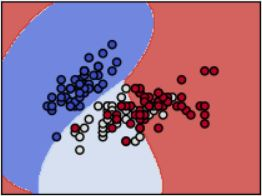
\includegraphics[width=.7\linewidth]{report_pics/SVM_RBF}
  \caption{RBF kernel}
  \label{fig:sub1}
\end{subfigure}%
\begin{subfigure}{.5\textwidth}
  \centering
  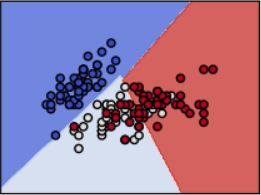
\includegraphics[width=.7\linewidth]{report_pics/SVM_linear}
  \caption{Linear kernel}
  \label{fig:sub2}
\end{subfigure}
\caption{SVM kernel types}
\label{fig:test}
\end{figure}

\subsection{K nearest neighbours}
Neighbors-based classification is a type of instance-based learning or non-generalizing learning: it does not attempt to construct a general internal model, but simply stores instances of the training data. Classification is computed from a simple majority vote of the nearest neighbors of each point. Under some circumstances, it is better to weight the neighbours such that nearer neighbours contribute more to the fit i.e. proportional to the inverse of the distance from the query point. As we would like to experiment with both options, we will create two KNN classifiers with two different distance functions and test their performance.
\begin{figure}[h]
\centering
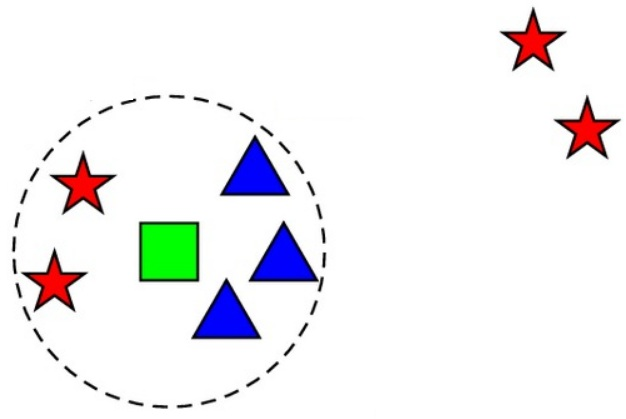
\includegraphics[width=0.3\textwidth]{report_pics/knn}
\caption{Classification depends on weight function}
\end{figure}
   
\subsection{Random Forest}
A random forest is a meta estimator that fits a number of decision tree classifiers on various sub-samples of the dataset and uses averaging to improve the predictive accuracy and control over-fitting. According to \href{https://medium.com/all-things-ai/in-depth-parameter-tuning-for-random-forest-d67bb7e920d}{medium.com post} the most important parameters of this classifier are:
\begin{enumerate}
	\item Number of trees - Usually the higher the number of trees the better to learn the data. However, adding a lot of trees can slow down the training process. Based on the experiments conducted in the post we decided to go with 50 trees.
	\item Maximum depth - represents the depth of each tree in the forest. The deeper the tree, the more splits it has and it captures more information about the data. The downside of a deeper tree, that it tends to overfit. Based on the post we chose to use maximum depth of 5.
	\item Minimum samples split - represents the minimum number of samples required to split an internal node. Large numbers will cause the nodes of the trees not to split at all disabling it's ability to learn. Thus we decide to use 0.1 value for this parameter.
\end{enumerate}

We find other parameters less important (and less intuitive), thus we will use the default values.

\subsection{Multi-layer perceptron}
Multi-layer Perceptron classifier. This model optimizes the log-loss function using LBFGS or stochastic gradient descent. In this section we discuss the most important parameters of MLP and the values we have chosen. Our decisions mostly based on the post in \href{https://stats.stackexchange.com/questions/181/how-to-choose-the-number-of-hidden-layers-and-nodes-in-a-feedforward-neural-netw}{stats.stackexchange.com}.
\begin{enumerate}
	\item Number of hidden layers - There is a consensus that the situations in which performance improves with a second (or third, etc.) hidden layer are very few. One hidden layer is sufficient for the large majority of problems. Based on this statement we decided to use only one hidden layer.
	\item Hidden layer size - There is rule of thumb that helps for supervised learning problems. The upper bound on the number of hidden neurons that will not result in over-fitting is:
\begin{gather*}
N_h = \dfrac{N_s}{\alpha * (N_i + N_o)}
\end{gather*}
while $N_o$ is number of output neurons, $N_i$ is number of input neurons, $N_s$ number of training samples and $\alpha$ is arbitrary factor between 2 and 10. In our case, for $\alpha = 10$
\begin{gather*}
N_h = \dfrac{7000}{10 * (16 + 13)} = 24
\end{gather*}
Causing most strict upper bound of 24 neurons in hidden layer. To prevent overfitting we will go with this number.
	\item Activation function - The default option is ReLU, but we would like to perform the experiment with Leaky ReLU as it has the same functionality but also prevents the "dead perceptron" phenomenon.
\begin{figure}[h]
\centering
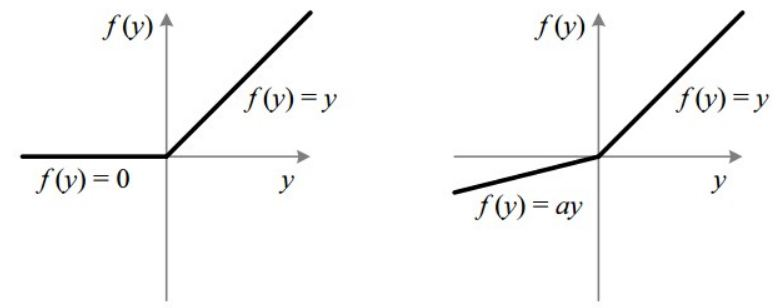
\includegraphics[width=0.5\textwidth]{report_pics/relu}
\caption{ReLU (left) and Leaky ReLU (right)}
\end{figure}
\end{enumerate}
We decided to leave other parameters at their default values as the problem of selecting the optimal neural network model is complex by itself and not should be covered in this submission. 


\newpage
\section{Performance measurements}
\subsection{Majority votes measurement}
For the task of prediction which party will win the majority of votes we propose to use the most simple measurement that comes to mind - "binary score": if the majority of predicted tags are from the same class as in validation set, the model score is 1, i.e. it has predicted correctly the winning party. Otherwise, the score will be 0, as the classifier predicted the wrong party. Those are the the only two possible values for this score, thus all models which got score 1 will be selected as best predictors for this task by the automated process in Selector class, while other models will be dropped.

\subsection{Votes division measurement}
For the task of prediction of votes division, we could use the "accuracy" or "error" measurement for the model performance, but we decided that those metrics are too strict for this task. In votes division task all we want is to predict correctly the division of the total votes (in test set) between the parties, but not a vote of each person. In other words, we want to compare a histogram of predicted votes to the histogram of true votes in the test set, thus the metrics we use is an Euclidean distance between two histograms:
\begin{gather*}
D = \sqrt[2]{\sum_{i=0}^{12} (histPredicted_i - histTrue_i)^2}   
\end{gather*}
According to this measurement, predicted votes distribution histogram which is very different form the true histogram, will be "far away" (in terms of Euclidean distance) from the true votes distribution histogram. On the other hand, predicted votes distribution histogram which is very similar to the true histogram, will be very close to it. Thus, the model with the shortest Euclidean will be considered as the best model for votes division prediction task.  

\subsection{Most probable voters measurement}
For the task of prediction of votes for each voter, we could use Average Accuracy. Based on 
\href{https://medium.com/usf-msds/choosing-the-right-metric-for-evaluating-machine-learning-models-part-2-86d5649a5428}{Choosing the Right Metric for Evaluating Machine Learning Models}, average accuracy is one of the most commonly used metrics for multi-class classification tasks. On the other hand, in this task we should predict a probability of each voter to vote for each party, but not the exact label. That's why we decided to use other metrics for this task. NOT FINISHED 
 

\newpage
\section{Prediction results and chosen model}
In this section we will discuss the results of each prediction task, the quality of the results according to the measurements and which model was selected for each prediction task.
\subsection{Majority votes}
To visualize the prediction results on validation set we will use histogram of true labels of validation set and predicted labels. According to those graphs we want be able to choose the best model for this task.

\begin{figure}[htp]
\centering
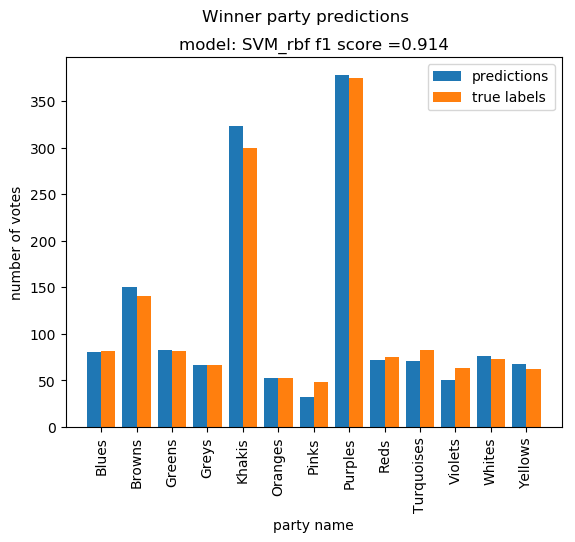
\includegraphics[width=.3\textwidth]{Winner_party_plots/SVM_rbf_fig}\quad
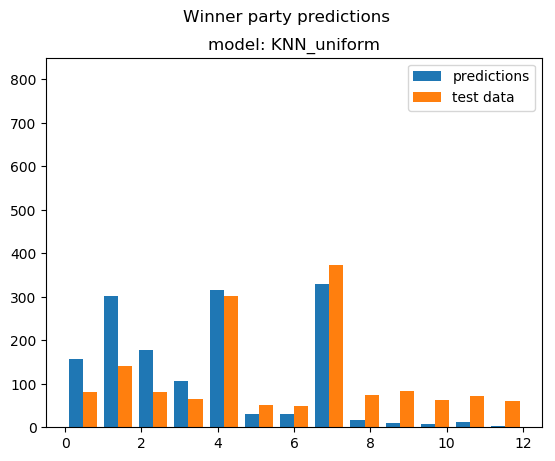
\includegraphics[width=.3\textwidth]{Winner_party_plots/KNN_uniform_fig}\quad
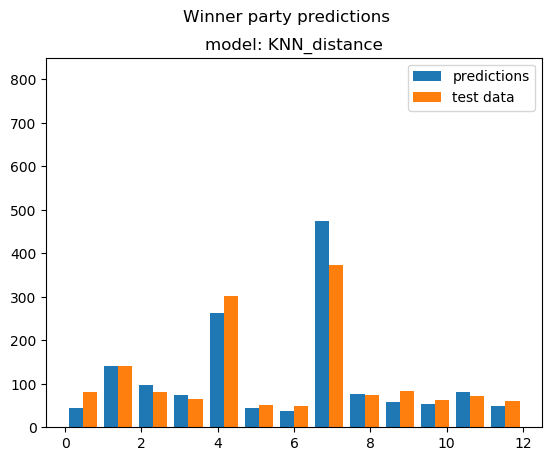
\includegraphics[width=.3\textwidth]{Winner_party_plots/KNN_distance_fig}

\medskip

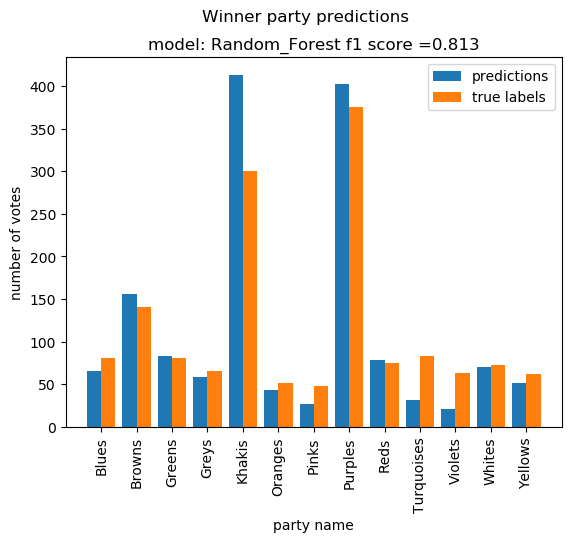
\includegraphics[width=.3\textwidth]{Winner_party_plots/Random_Forest_fig}\quad
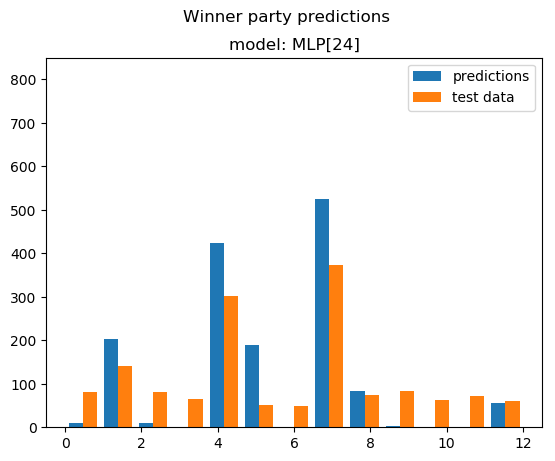
\includegraphics[width=.3\textwidth]{Winner_party_plots/MLP[24]_fig}

\caption{Votes distribution}
\end{figure}

Looking at the plots we can say that all five models predicted the winner party correctly. On the other hand, during the experiments we noticed that MLP votes distribution changes each time we train the network from scratch. To make MLP results consistent we forced to add the same random state each time we initialize the network weights, which is, of course, not a real solution to this issue. At this point we definitely can drop MLP from this task. Other four predictors successfully predicted the winner party, while SVM did it with the highest level of certainty, i.e. the majority of the samples where classified according to the real tag majority in the train set. As the class proportions in training, validation and test sets are the same, SVM probably will give the same prediction on the test set.
  
\subsection{Votes division}
To visualize the prediction results on validation set we will use histogram of true labels of validation set and predicted labels. According to the metrics we choose for Votes division task, we are interested in model which achieved the smallest Euclidean Distance between the histograms. 


\begin{figure}[htp]
\centering
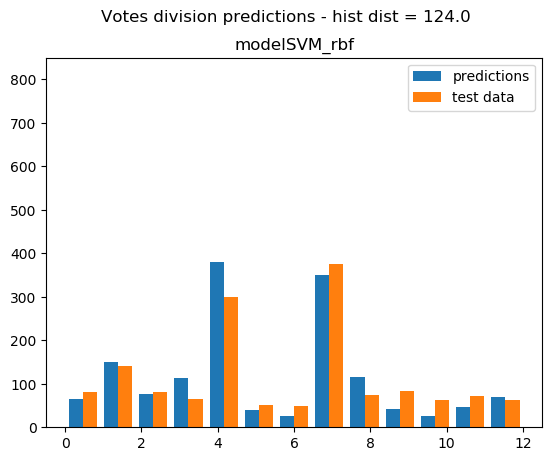
\includegraphics[width=.3\textwidth]{Division_prediction_plots/SVM_rbf_fig}\quad
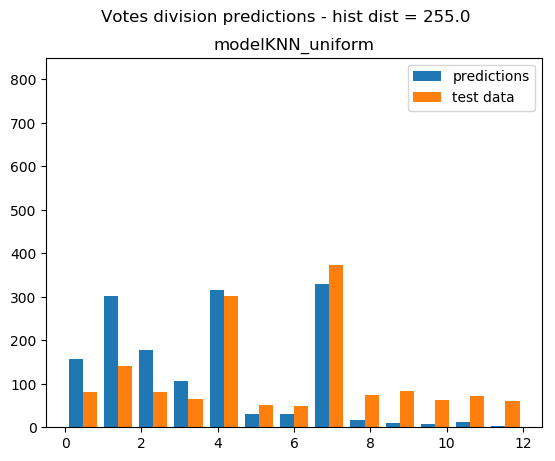
\includegraphics[width=.3\textwidth]{Division_prediction_plots/KNN_uniform_fig}\quad
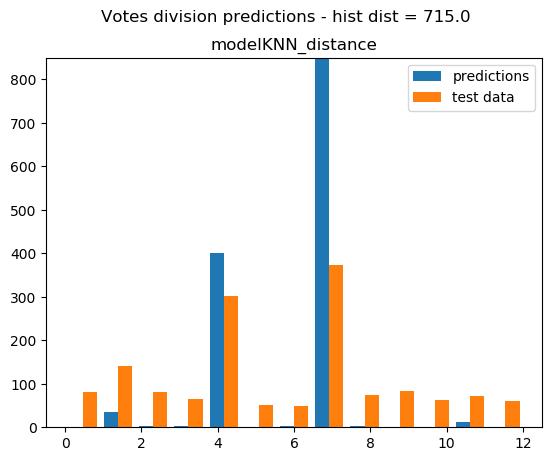
\includegraphics[width=.3\textwidth]{Division_prediction_plots/KNN_distance_fig}

\medskip

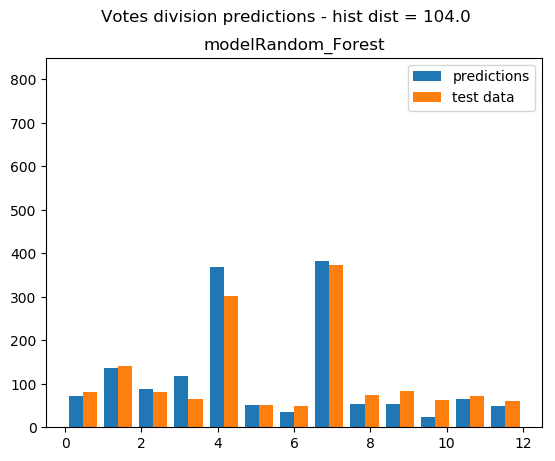
\includegraphics[width=.3\textwidth]{Division_prediction_plots/Random_Forest_fig}\quad
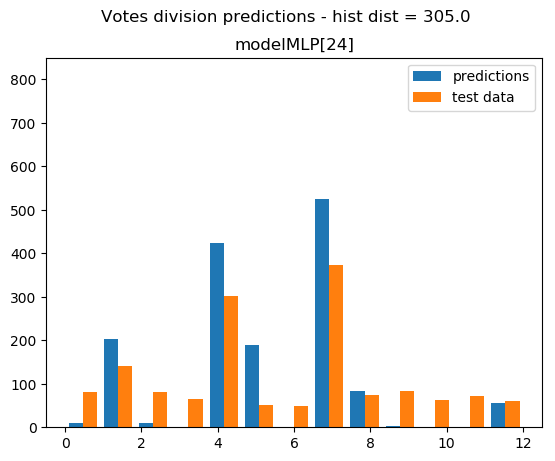
\includegraphics[width=.3\textwidth]{Division_prediction_plots/MLP[24]_fig}

\caption{Votes distribution}
\end{figure}

Looking at the plot we can clearly see that model performance corresponds to the chosen metrics, i.e. the euclidean norm. As stated in previous sections, the most similar histograms have the smallest euclidean distance. In conclusion, KNN classifier with weighted distances achieved best performance on validation set with final score of 120, which is the best score among other classifiers. 

\subsection{Vote per voter}

\newpage
\section{Final answers}
\subsection{Which party will win}
\subsection{Votes division}
\subsection{Most probable voters}
\subsection{Confusion matrix}

\newpage
\section{Discussion}
\subsection{Comaring results of validation set vs test set}
\subsection{A}
\subsection{B}
\subsection{C}

\begin{enumerate}
	\item one
	\item two
\end{enumerate}

\end{document}
